\chapter{面向隐私保护的风险自适应访问控制模型}
\label{chap:RaBAC-for-privacy}

\textit{ }

\textit{本章针对云环境中共享、应用涉及隐私或敏感信息数据的场景研究面型隐私保护的访问控制模型。在此类以数据为中心的开放跨域环境,大量用户以不同形式的应用需求来访问数据,数据拥有者(即数据服务提供者或系统)需要动态化、自适应的提供隐私保护。我们在XACML上扩展提出了一种基于风险的自适应访问控制模型,以动态化在访问控制过程中保护数据隐私,约束隐私侵犯行为,激励诚实访问行为。在该模型中,以Shannon信息论作为工具,在第\ref{chap:entropy-metric-model}章提出的隐私度量度量模型基础上,提出了基于风险的隐私定义和量化方法;通过风险隐私量化及基于信誉的激励机制,实现访问行为风险阈值的动态调整。对比和分析表明,所提出的模型和方法较现有的工作更加动态化,且实现了隐私保护,易用性更好。本章成果已发表在《International Journal of High Performance Computing and Networking》。
}
\section{概述}
\label{sec:intro}
随着云计算的发展和云计算模式的广泛应用,越来越多的敏感数据和隐私信息在云环境中存储、应用,致使云面临着若干安全问题。云计算环境中的隐私、机密性和完整性等身份识别与访问控制相关的安全性需要保证。访问控制模型对云安全极为重要,但云中仍然在大量应用传统的访问控制,而这些方案存在不同层面的安全和隐私问题。
传统访问控制模型,例如ACL (访问控制列表) \cite{qian2001acla}, RBAC (基于角色的访问控制) \cite{jung2012cribac}, ABAC (基于属性的访问控制) \cite{zhang2011attribute}和PBAC (基于策略的访问控制) \cite{huang2011policy} 是严格和静态的访问控制模型, 需要管理员预定义所有访问策略。 在像云环境这样的“按需共享”的大规模信息系统中,用户和资源都是动态的且一直在变化,不可能预先定义访问策略,而传统的访问控制方法无法适应这种情况。

为了解决此问题,基于风险的访问控制\cite{ni2010risk,shaikh2012dynamic,wang2011quantified,choi2015framework}被引入,因为其将风险级别分析作为授权决策过程的主要输入,以实现动态访问控制。基于风险的访问控制通过考虑访问请求的环境和情况以及安全策略来评估风险,并根据阈值确定访问权限。这种决定访问权限的方式可以通过反映情况的本质并防止由于内部人员滥用和滥用数据而导致不必要的隐私信息访问和泄漏,从而实现动态访问控制 \cite{chen2011risk}。 因此,风险量化成为基于风险的访问控制中的核心组件。

一般情况下风险定义为潜在的资源价值损失。在信息系统中,访问风险可以被视为因访问数据所可能造成的潜在泄露信息价值。现有以基于风险的访问控制研究进展提供了不同的方法来确保访问对象的安全性和隐私。Chen等\cite{cheng2007fuzzy} 提出了一种模糊多级风险访问模型,该模型采用模糊理论来评估对象的通行等级和对象敏感度等级对,随后Ni等\cite{ni2010risk} 将Chen等的思想思想扩展为基于模糊推理的访问控制。Wang和Jin\cite{wang2011quantified} 在健康信息系统的访问控制中提出了一种基于条件熵的风险量化方法,以保护患者的隐私。Shaikh等\cite{shaikh2012dynamic}提出了一种基于动态风险的访问控制系统决策方法的新方法,同时考虑了短期历史访问行为和长期历史访问行为。Khambhammettu等\cite{khambhammettu2013framework} 将威胁资源和低手影响考虑至访问请求风险量化中,并以此提出了一个访问控制模型的风险量化方法。Choi等\cite{choi2015framework} 对上下文信息进行了分类,通过扩展可扩展的访问控制标记语言 (XACML) 来应用风险,从而通过基于上下文和处理的权限配置文件和规范来估计和应用风险。但是这些工作都需要使用相同的方法来对访问主体(用户) 和访问客体 (资源或信息)进行分类, 且在特定情况下很难找到这种方法。尽管现有工作可以动态地基于风险来决定访问许可,但是其最大可容忍风险值 (风险阈值) 是静态的,对于所有用户而言都是相同的容忍度,且缺乏对访问主体的激励机制。

本章目针对上述问题,提出了一种基于马尔可夫和信息论的风险自适应访问控制模型。首先,为基于风险的访问控制模型定义了一个敌手模型,提出了一些自然而有用的假设和定义,仅通过比较访问行为模式即可对访问请求和用户进行分类。然后,提出了一种基于XACML的风险自适应访问控制框架。在此框架中,添加了策略风险评估点 (Policy Risk Evaluator Point, PREP), 会话控制和风险缓解服务三个新组件,并增强了策略执行点,策略访问点和策略信息点三个标准组件。针对PREP设计了基于类马尔科夫的公式和方法,以根据访问历史行为来计算访问请求的风险值,基于请求类别识别来允许/拒绝访问请求,并根据访问历史周期性计算用户风险,并设计激励机制通过重新定位风险配额和风险消耗配额。

\section{相关工作}
\label{sec:relate}
最近,基于风险访问控制模型吸引了研究人员的注意\cite{wang2011quantified,shaikh2012dynamic,choi2015framework}。Wang和Jin\cite{wang2011quantified} 考虑了一种实际的访问控制模型,该模型通过考虑医疗保健的实际情况来保护电子医疗系统中的患者隐私。首先,该模型允许医生通过量化与医生的数据访问活动相关的风险来做出访问决策。其次,该模型利用医生的整体统计行为和Shannon条件熵来量化侵犯隐私的风险。Hui等\cite{hui2015risk}改进, 对此模型进行了改进,但是两个模型都不能在近期历史和旧历史之间取得平衡,也没有采取任何措施来减轻高风险。Shaikh等\cite{shaikh2012dynamic} 提出了一个用于访问控制系统的基于动态风险决策方法。首先,其改进了标准XACML框架,添加了策略风险和信任评估者点。其次,系统根据奖励和惩罚历史计算主体的信任值和客体的风险值。此外,该系统通过使用基于指数加权移动平均值 (EWMA) 的方法来考虑近期历史和旧历史的不同影响。 最后,分析了允许非法访问和限制合法访问的威胁。该系统可以根据过去的行为自适应并适度增加或减少所有用户对资源的访问权限,但是访问主体和访问客体需要相同的分类方式进行标记。此外,该系统仅根据主体-客体间奖励或惩罚点做出访问决策,没有针对访问主体历史行为的奖励机制或惩罚机制。Choi 等\cite{choi2015framework}  提出了一种适用于医疗信息系统的基于风险的访问控制框架,以保护患者的敏感数据和隐私。该方法的主要思想是根据医疗情况和处理的严重性,通过动态访问授权决策来估计和应用风险。在对有关医生的目的,患者的状况和治疗以及医疗数据的上下文信息进行分类之后,可以根据特定患者的状况和治疗的条件下访问请求与目的之间的相关性来评估风险等级。尽管该模型可以在某些严重情况下授予访问权限,但其并未提供缓解高访问风险的措施,使得在后续访问过程造成风险量化混乱。

我们提出的方法与\cite{wang2011quantified,shaikh2012dynamic,choi2015framework}等文献的方法相比,具有一些新的特性。

\begin{enumerate}
	\item 该方法中,资源所有者或访问控制系统的管理员只需标记或分类访问对象(例如,资源,存储的数据,数据等) 根据访问对象的属性和要求,通过某些标准方法(例如,用于病历的IDC-10) 或定制方法。不需要为访问主体 (例如,经过身份验证的用户) 特定明确的角色或工作职责,也无需为每个访问请求特定目的。
	\item 访问主体的工作职责是通过对主体历史访问数据聚类而得到的,且将访问主体划分为不同的非相交组。
	\item 基于类马尔可夫模型设计了访问请求风险值计算,用户风险值计算,不同组中用户的迁移等方法。
	\item 设计了一种类似于信用卡的激励机制,对主体的所有访问行为进行监督,并通过这种机制约束了风险请求和风险用户。
\end{enumerate}

\section{基本定义和敌手模型构建}
\label{sec:adversary_model}

本节进行若干假设和定义,并此提出基于风险访问控制模型的敌手模型。如第~\ref{sec:intro}节所述,本章主要聚焦对信息系统中经过身份验证的用户的访问行为控制,以保护敏感数据和隐私。在此类系统中,所有用户,包括敌手,都被授权使用存储的数据,本章的目的是防止用户不履行其在系统中的职责时,访问不该访问的敏感或隐私数据而造成的隐私泄露。

\begin{assumption}
	\label{ass:user_obligations}
	所有通过身份验证的用户都将履行其职责。
\end{assumption}

若用户通过了特定信息系统的认证,则他为合法用户,且他有责任履行其工作职责。一旦对员工没有足够的工作职责,系统将不会容忍用户。此外,若用户未履行其工作职责,则不会对敏感或隐私数据造成太大伤害。 根据假设 ~\ref{ass:user_obligations},可以将经过身份验证的用户分为几类, 即\emph{诚实用户}和\emph{好奇用户}, 有时将\emph{好奇用户} 认为是 \emph{恶意用户}。 \emph{诚实用户} 仅访问其职责所需的数据或信息,  \emph{好奇用户} 有时会故意或随机访问与其职责无关的敏感或隐私数据或信息,但与\emph{诚实用户}相同的访问行为除外。 只有当\emph{好奇用户}故意访问与工作职责无关的敏感或隐私数据或信息时,其才被称为 \emph{恶意用户}。方便起见,在本章的研究中,对这两个概念的不加以区别的对待。

\begin{assumption}
	\label{ass:honest_user}
	大多数通过身份验证的用户都是诚实用户。 相应地,只有一部分经过身份验证的用户是好奇用户或恶意用户。
\end{assumption}

假设~\ref{ass:honest_user}在现实环境中是合理的。 现实中的大多数人都是好人,否则我们的社会将会混乱。假定部署在云或本地设备中的任何信息系统都有序运行,且大多数用户都是诚实的。一旦\emph{好奇用户} 被系统识别,可以通过惩罚或拒绝好奇的用户来确保这一假设。

对于经过身份验证的特定用户,还可以根据访问请求的风险值将其访问行为分为两类。 一部分行为具有较高的风险值,而另一部分行为具有较低的风险值。 该分类由以下事实决定:没有绝对的分类,即所存储的信息和数据中哪些与该用户的职责有关,哪些与该用户的职责无关。 我们的目的是将 \emph{好奇用户} 与\emph{诚实用户}区分开, 拒绝 \emph{好奇用户}, 并减少\emph{诚实用户}的偶然高风险行为对\emph{诚实用户}的访问控制决策的影响。为了实现该目标,需实现以下内容:

\begin{enumerate}
	\item 根据身份验证用户的工作职责将其分为几组,且每两个组的交集在一段时间内为空;
	\item 识别每个用户的职责变更,并将变更后的用户分别分组为适当的组;
	\item 评估每个用户的每个访问请求的风险,并识别具有高风险值的请求;
	\item 定期评估每个用户的风险,识别好奇的用户并拒绝他们。
\end{enumerate}

以上表明同一组中的所有用户都具有相似的工作职责,因此,若 $u \in g$ ,则不区分用户 $u$ 和组 $g$ 的职责。在提出的敌手模型中,在特定的用户组中,对于访问行为,若该访问请求的访问数据蕴含隐私信息比历史访问行为多,则访问行为具有高风险。为了对高风险请求和正常请求的风险评估建模,引入两个假设函数,即 $sr$ \emph{自我风险函数}和$gr$ \emph{组风险函数}。 其中,$sr(u,q)$ 表示用户 $u$的当前访问请求 $q$ 对 $u$自身的历史访问行为的风险值,  $gr(u,q)$ 表示风险值$u$的用户当前访问请求 $q$中$u$ 所属用户组 $g$ 的历史访问行为。$sr(u,q)$ 和 $gr(u,q)$ 的具体计算公式将在 \ref{sec:proposed model}中讨论。

\begin{definition}%[Self Risky Request and Self Normal Request]
	\label{def_self_risky}
	令 $sr(u, q_0), sr(u, q_1), sr(u, q_2), ... ,sr(u, q_{n-1})$ 为过去 $n$ 次请求 $u$ 的自风险值, 令 $sr(u,q)$ 为 $u$ 当前 (第n次) 请求 $q$ 次的风险值。 令 $\epsilon_s \in (0,1)$ 为分位数。若$sr(u,q) \geq  (1+\epsilon_s) / n  \sum ^{n-1}_{i=0}\\{sr(u,q_i))}$,则请求 $q$ 是一个\textbf{用户自风险请求}。否则, $q$ 是一个 \textbf{用户自我正常请求}。
\end{definition}

\begin{definition}%[Group Risky Request and Group Normal Request]
	\label{def_group_risky}
	令 $gr(\cdot, q_0), gr(\cdot, q_1), gr(\cdot, q_2), ... , gr(\cdot, q_{m-1})$ 是过去 $m$ 的组风险值乘以同一用户 $u$ 组中的用户请求。并将 $gr(u,q)$ 设为用户 $u$ 的当前请求 $q$  ( $u$ 所属组的第m个请求 )。 令 $\epsilon_g \in (0,1)$ 为分位数。若$gr(u,q) \geq  (1+\epsilon_s) / m  \sum ^{m-1}_{i=0}{sr(\cdot,q_i))}$,则 $u$ 的请求 $q$ 是一个\textbf{组风险请求}。否则, $u$ 的 $q$ 是一个 \textbf{组正常请求}。
\end{definition}


上述定义 \ref{def_self_risky}和定义\ref{def_group_risky} 都基于马尔可夫模型,且可以根据访问控制系统的经验自动确定马尔可夫链的长度。 此外,两个长度都可以随时间变化。通过这两个定义可以有效识别访问控制系统的高风险访问请求。具体详细计算方法,将在第\ref{sec:proposed model}节中详细讨论。 在一个时间段内,特定组的每个用户的请求数据数据的期望服从某些分布,而该组的所有用户请求的数据数据的期望也服从一定的分布。根据假设 \ref{ass_honest_user}, 若 $u$ 是一个诚实的用户,则用户 $u$ 的访问数据的分布 $D_u$ 与同一组中所有用户访问的数据的分布 $D_g$ 密切相关。相反,若 $u$ 是一个好奇的用户,则 $D_u$ 与 $D_g$ 无关。 为了有效描述这种关系, 引入 \emph{相关关系函数} $\theta$ 并将在 第\ref{sec:proposed model}节中进行讨论。对于用户 $u$ 在组 $g$ 中通过请求 $q$ 访问的数据数据集合 $r$,$\theta_g (r_q,u))$ 返回一个 [0,1]的实数,该实数反映 $r_q$ 和 $u$ 的职责之间的相关程度,$\theta_g (r_q,u))$ 越高, 风险$r_q$ 对于用户 $u$ 的职责而言就越高。


\begin{definition}%[Honest User and Curious User]
	\label{def_curious user}
	假定 $D_g$ 是特定组 $g$ 的所有用户 $U_g$ 访问的数据数据集合 $R_g$ 的先验概率分布,$D_g$ 使得 $Pr(R_i)=\delta \cdot \theta_g (\cdot,u_i))$,其中 $u_i$ 是 $g$ 中的用户, $R_i$ 是 $u_i \in g$ 访问的数据数据集合,而 $\delta$ 是实数,因此 $\Sigma_{u_i \in g}Pr(R_i) = 1$。
	\begin{itemize}
		\item \textbf{诚实用户}: 设 $R_i$ 为 $u_i \in g$ (即诚实用户) 在过去一段时间内访问的数据集, 对于每个数据 $r_k \in R_i$, 概率为 $(1-\epsilon_1)$ 时,  $r_k$ 的选择遵循 $D_g$ 分布 ; 概率为 $\epsilon_1$ 时,  $r_k$ 的选择遵循 $R_g$ 所有可用数据的均匀分布, 其中 $\epsilon_1 \in [0,1]$.
		\item \textbf{好奇用户}: 设 $R_i'$ 是 $u_i' \in g$ (即好奇用户) 在过去一段时间内访问的数据集, 对于每个数据 $r_k' \in R_i'$, 概率为 $(1-\epsilon_1)(1-\epsilon_2)$ 时,  $r_k'$ 的选择遵循 $D_g$ 分布 ; 概率为 $\epsilon_1 (1 - \epsilon_2)+ \epsilon_2$,  $r_k'$ 的选择遵循 $R_g$ 所有可用数据的均匀分布, 其中 $\epsilon_1, \epsilon_2 \in [0,1]$.
	\end{itemize}
\end{definition}

如定义\ref{def_curious user} 所述, 诚实用户的数据访问始终遵守其职责 (即,用户总是遵循分配 $D_g$), 例外情况的发生概率小于 $\epsilon_1$. 相反,好奇用户的行为与诚实用户的行为以概率$1-\epsilon_2$ 相同, 他履行了自己的职责;好奇用户以概率 $\epsilon_2$ 过度访问敏感数据。在真实场景中,$\epsilon_1$ 和 $\epsilon_2$ 的值都较小。

\section{所提出的风险访问控制模型}
\label{sec:proposed model}
本节根据可扩展访问控制标记语言 (XACML) \cite{verma2004xml} 改进提出一个风险自适应访问控制模型,然后提出如何初始化访问控制系统,如何定义并量化访问请求风险,如何为请求做出访问决策,访问控制过程详细过程、如何动态识别好奇用户,以及如何设计激励机制等具体方法。

\subsection{风险访问控制模型框架}
\label{subsec:framework}

在标准XACML框架中,一旦策略决策点 (PDP) 收到了来自访问主体 (即访问控制系统的用户) 的访问请求, 其首先会从策略访问点 (PAP) 和策略信息点 (PIP) 然后决定接受还是拒绝该请求。 此外,策略执行点 (PEP) 难以处理与请求者的交互,策略访问点 (PAP) 是静态的,且职责服务和策略信息点 (PIP) 都缺乏风险管理。
在我们提出的框架中,除了对PEP,PIP和PAP进行了增强,还新增了三个组件,即策略风险评估点 (PREP),会话控制和风险缓解服务 (嵌入在职责服务的组件中)。 在该框架中,一旦PDP收到来自经过身份验证的用户的访问请求,且在做出决定之前,它会请求与特定访问主体 (即正在请求访问的用户) 和其历史访问数据相关的风险值。此外,在做出访问控制决策后,一些反馈信息将提供给职责服务。 所提出的风险自适应访问控制模型的流程如图~\ref{fig:Process_flow}所示。 该框架是基于标准可扩展访问控制标记语言 (XACML) 提出的,与 \cite{shaikh2012dynamic}的框架有所不同,所提出框架的所有新组件均以虚线标记,所有增强的组件均浅灰色标记。


\begin{figure}[htbp]
	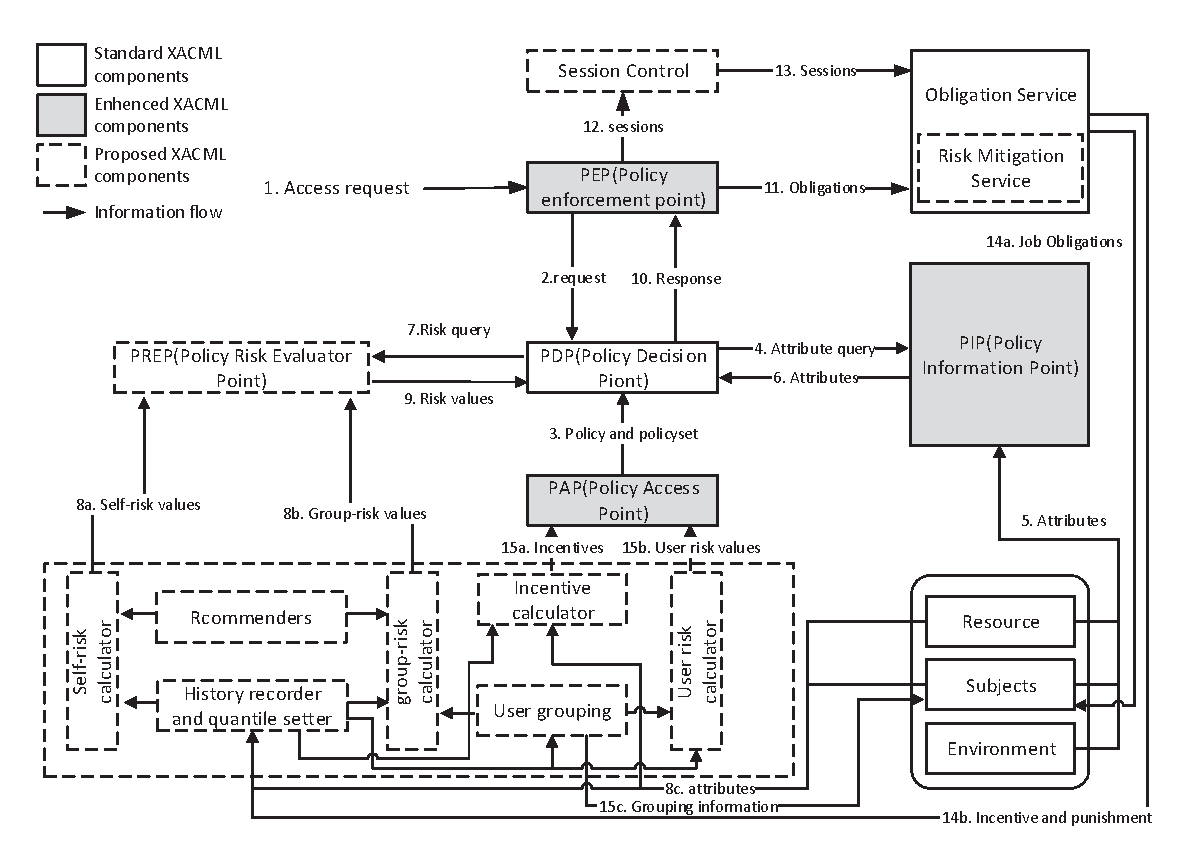
\includegraphics[width=\linewidth]{./figures/Process_flow.eps}
	\caption{基于XACML的风险自适应访问控制模型处理流程}
	\label{fig:Process_flow}
\end{figure}

在所提出的基于标准XACML风险访问控制框架中,所有访问请求均由经过身份验证的用户发送,我们称此类用户为访问主体。 从步骤1到步骤6,其过程类似于Shaikh等\cite{shaikh2012dynamic} 和Verma \cite{verma2004xml}所述的过程。一旦收到所有必需的信息,PDP就将有关当前请求的风险查询发送到PREP (步骤7)。 PREP根据用户的过去行为和历史行为的风险值来评估风险值 (步骤 8)。 每个请求都有两个风险值,一个是根据当前用户自己的过去行为评估的自我风险值,另一个是根据所有用户的过去行为以及当前用户属于同一组所有用户评估的群组风险值。
若系统没有足够的历史数据,则PREP将根据系统平均风险水平评估两个隐私风险值。与该访问请求相关的当前风险值将返回到PDP (步骤 9)。根据风险值,PDP做出决定,并将此决定转发给PEP,由PEP执行 (步骤10)。无论是允许访问还是拒绝访问,PEP都会通知 (步骤 11) 职责服务,该服务将决定是否需要风险缓解服务。在强制执行的延迟时间内,会话控制组件监视请求者的行为,并管理访问会话 (步骤 12)。若在该会话中访问行为的隐私风险太高,则会话控制通知职责服务组件并控制该会话中的请求 (例如,终止会话) (步骤 13)。 职责服务将决定是激励还是惩罚用户,并更新主体的属性 (例如工作职责) (步骤 14)。 PREP定期通过激励机制重新分配预算配额,重新将用户标识为正常用户或有风险的用户,并将用户分类到为更合适的群组中(步骤 15)。

\subsection{请求风险值和请求决策}
\label{subsec:risk values and decision}
\subsubsection{请求风险值}
本章中,动态评估访问请求风险值的方法是根据请求者的过去行为以及基础请求者所属组的所有成员而设计的。对于特定的用户组,该组中的每个用户都按照相似的工作职责划分到该组中,其工作职责在短时间段内相对稳定,且会在长时间周期范围自然演变。对于特定的用户,其所属的组可能会随时间改变。因此,应该根据用户本人和组的短时间访问行为特征来评估特定组中用户的访问请求风险,可以根据用户本人和组的长时间访问行为特征来识别用户风险。本节仅关注对特定用户的访问请求隐私风险评估。直观地,一访问请求的目的是访问一个时间周期内没有被访问过的数据数据集,则即使该数据数据集在以前被该用户访问过,该请求的访问请求的隐私风险值也很高。我们将该思想应用于对访问请求的隐私风险评估中,基于信息论相关概念,并对其进行改进,以设计本章用以进行访问请求隐私风险值量化的函数。

令 $u \in U$ 是已认证用户集 $U$, 且 $u$ 属于用户组 $g$ ,该用户组$g$ 是 $U$ 的子集。 如定义 \ref{def_self_risky} 和 \ref{def_group_risky}所述,$u$ 的请求 $q$ 有一定的隐私风险,表示为 \emph{用户自风险} $sr$ 和 \emph{组风险} $gr$ 。

令 $(q_1, q_2, ... , q_{n-2}, q_{n-1})$ 为用户$u$的前$n-1$次访问请求,而 ${r_1, r_2, ... , r_{n-2}, r_{n-1}}$ 分别为这些请求的访问数据集。 令 $q_n$ 是用户当前的访问请求,该访问请求所要访问的数据集为 $r_n$。若将每个访问请求和访问数据集对 $(q_n,r_n)$ 视为随机事件,则该对 $(q_i,r_i)$ 的信息量可以通过\textbf{自信息}表示。则当前访问请求的访问隐私自风险 $sr$ 可表示为

\begin{equation}
\label{eq:self risk}
sr(u,q_n)=I(q_n,r_n)
\end{equation}

由公式\ref{eq:self risk} 中可知, 可由$r_n$ 中预期访问的数据集的概率分布计算得到$rs$。此外,由于不同的数据集具有相同的标签,因此其可能具有相同的敏感信息。 故而,在不同的情况下应使用不同的分类方法对数据进行标签化分类。 可以将关系数据库中的数据分类为相同的数据,以使这些数据具有相同的信息;在电子医疗信息系统中,具有相同信息的医疗数据应按标签分类 (例如ICD-9或 ICD-10代码)。

为方便起见,后文将不再对访问请求 $q$ 和其预期访问的数据集 $r$ 进行区分, 即,每个不同的访问请求都试图访问具有不同信息的不同数据。 假设访问请求集 $Q_u$ 中有 $k$ 个不同的请求 $q_1,q_1,....,q_k$ ,其中包括前$n-1$ 次访问请求和的 $u$ 的当前访问请求 $q_n$ ,以及概率分别为 $p_1,p_2,...,p_k$ 。 若在 $k$ 个不同的请求中 $q_n$ 与 $q_i$ 相同,则方程 \ref{eq:self risk} 可以简化为

\begin{equation}
\label{eq:self risk 2}
sr(u,q_n)=I(q_i)=-logp_i
\end{equation}

公式 \ref{eq:self risk} 和 \ref{eq:self risk 2} 都在具有足够的历史访问请求行为时,才对用户$u$ 有效,若无有足够的历史访问行为历史供 $u$进行计算, 则可以使用某个默认值 (例如1) 或整个历史数据。
	\begin{equation}
	\label{eq:self risk 3}
	sr(u,q_n)=
	\left\{
	\begin{array}{ll}
	I(q_i)=-logp_i, & \hbox{是否有足够的历史数据;} \\
	Avg(I(u,q)), & \hbox{若历史还不够;} \\
	1, & \hbox{若没有可用的历史数据。}
	\end{array}
	\right.
	\end{equation}

由公式\ref{eq:self risk 3}可知,$rs$ 的计算依赖于用户 $u$ 自己过去 $n-1$ 次访问行为的马尔可夫链,且马尔科夫链的长度可以根据需要针对每个用户进行动态和个性化设置。这样,可以通过调整参数~$n$~的大小,适当地平衡用户 $u$ 的短期历史和长期历史行为对隐私风险值的影响。

令 $sr(u, q_1), sr(u, q_2), ... , sr(u, q_{n-2}), sr(u, q_{n-1})$ 为过去 $n-1$ 次允许请求 $u$ 的隐私自风险值,并令 $sr(u,q)$ 为 $u$ 当前 (第n次) 请求 $q$ 的当前访问请求的隐私自风险值。令 $\epsilon_s \in (0,1)$ 为分位数, 通过定义 \ref{def_self_risky} 可以方便地将$q$ 定义为 \textbf{自风险请求} 或 \textbf{自正常请求} 。

类似地,可以通过该马尔可夫方法得到当前用户 $u$ 的当前访问请求的组风险值。 令 $q_1,q_1,....,q_l$ 是访问请求集 $Q_g$ 中的元素,它表示组 $g$ 过去的 $m-1$ 次允许访问请求和 $u\in g$ 的当前访问请求 $q_m$, $p_1,p_2,...,p_l$ 分别为历史访问请求数据集的标签化概率分布。 若 $q_m$ 与 $Q_g$ 中的 $q_i$ 相同, 则 $gr(g,q_m)$ 可计算为
	\begin{equation}
	\label{eq:group risk}
	sr(g,q_m)=
	\left\{
	\begin{array}{ll}
	I(q_i)=-logp_i, & \hbox{若有足够的历史数据 ;} \\
	Avg(I(g,q)), & \hbox{若历史还不够;} \\
	1, & \hbox{若没有可用的历史数据。}
	\end{array}
	\right.
	\end{equation}
类似地,通过定义 \ref{def_group_risky} 可将 $u\in g$ 的访问请求 $q$ 识别为 \textbf{组风险请求}或\textbf{组正常请求} 。


\subsubsection{访问控制决策}
自风险值 $sr(u,q)$ 和组风险值 $gr(g,q)$ 都是访问决策的基础。 根据定义 \ref{def_self_risky} 和 定义\ref{def_group_risky}, 可将所有用户的访问请求分为四类,即访问请求 $q$ 有四个不同的风险级别。故,数据服务提供者或系统可以根据请求的风险级别做出访问控制决策,即
\begin{equation}
	\label{eq:decision}
	decision=
	\left\{
	\begin{array}{ll}
	p, & \hbox{若$q$为自正常访问请求,且为群组正常访问请求;} \\
	p(rm), & \hbox{若$q$为自风险访问请求,但为群组正常访问请求;} \\
	d, & \hbox{若$q$为自风险访问请求,且为群组风险访问请求;} \\
	d(p), & \hbox{若$q$为自正常访问请求,但为群组风险访问请求。} \\
	\end{array}
	\right.
\end{equation}
其中,$p$表示因为访问请求时正常的,访问请求没有隐私风险,授权该访问请求;$p(rm)$ 表示该访问请求隐私风险较低,用户通过一定风险消减措施之后,可以授权该请求进行数据访问;$d$ 表示由于该访问请求隐私风险过高而拒绝访问;$d(p)$ 表示该访问请求隐私风险太高,应当惩罚并限制用户访问包含隐私的敏感数据集。

公式\ref{eq:decision}中对访问请求的访问控制决策的确定基于以下原因。 若请求既是自身正常请求又是组正常请求,则用户和组在过去一段时间内频繁访问该访问请求的请求访问数据集,因此该请求是正常的而且没有风险。 若某个请求是自风险请求,且是组正常请求,则表示该组中的其他用户(非用户本人)经常访问了预期数据,这些数据与该组的工作职责相关,但用户几乎不访问,且对该用户的访问风险很小,应该在系统采取某些适当的风险缓解措施后授予访问权限。若某个请求是自风险请求,且是组风险请求,则该组几乎不会访问预期数据,这些数据与该组的工作职责无关,因此访问请求应被拒绝。若某请求是一个自正常请求,且是一个组风险请求,则该组几乎不会访问预期数据,且这些数据与该组的工作职责无关,但该用户已多次访问数据,因此应拒绝访问此请求,并要加重惩罚以限制该用户访问。


\subsection{用户分类与激励机制}
\label{subsec:User classification and incentive mechanism}
本节首先基于用户和用户组历史访问请求,提出可定期地将用户 $u \in g$ 识别为好奇用户还是诚实用户的方法。然后,提出可定期确定用户如何从一个组迁移到另一个组的方法; 最后,设计了一种激励机制,以监督用户访问行为,抑制风险请求和风险用户。特别地,本节的所有方法,都基于类马尔科夫模型和信息论。

\subsubsection{用户的风险值和用户分类}
对于特定用户组中的用户,可在假设 \ref{ass:user_obligations}和假设 \ref{ass:honest_user} 下通过定义 \ref{def_curious user} 将用户识别为好奇用户或诚实用户。但实际上很难找到 $\theta_g$ 的特定函数,我们通过使用组 $g$ 的访问模式来近似刻画函数 $\theta_g$ 。信息熵可用来表示信息集的不确定性,故而我们采用香农熵来表示组和用户的访问模式,用户访问行为的熵越高,用户越好奇。

令 $T$ 为周期时间, $Q_{g,T}=(q_1, q_2,...,q_{s_g})$ 为 $T$ 中 $u$ 组所有用户的访问请求, $Q_{g,T}$ 遵循分布
$P(g,T)=
(
\begin{array}{l}
q_{g,1},  q_{g,2}, ...,q_{g,n_g}\\
p_{g,1},  p_{g,2}, ...,p_{g,n_g}\\
\end{array}
)
$。令 $Q_{u,T}=(q_1, q_2,...,q_{s_u})$ 为 时间$T$ 中来自用户 $u \in g$ 的访问请求, $Q_{u,T}$ 遵循分布
$P(u,T)=
(
\begin{array}{l}
q_{u,1},  q_{u,2}, ...,q_{u,n_u}\\
p_{u,1},  p_{u,2}, ...,p_{u,n_u}\\
\end{array}
)
$。

然后可以计算出用户 $u \in g$ 在时间段 $T$ 中的风险值 $risk(u,T)$ 为
\begin{equation}\label{eq:user risk}
risk(u,T)=max \{\frac{H(P(u,T))-H(P(g,T))}{H(P(g,T))},0\}
\end{equation}
其中,等式 \ref{eq:user risk}表示在过去的时间段 $T$ 中,用户风险随熵的增加而线性增加。但实际上,始终存在阈值 $\phi$, 使得用户A和用户B的风险相似, 当 $H(P(A,T))>H(P(B,T))>\phi$ 时,甚至 $H(P(A,T))-H(P(B,T))$ 非常大。然后可以将公式 \ref{eq:user risk} 中的风险值计算改进为
\begin{equation}\label{eq:user risk 2}
risk'(u,T)=\alpha ^ {max \{H(P(u,T))-H(P(g,T)),0\}}
\end{equation}
其中, $\alpha \in (0,1)$, 而风险的结果 $risk'(u,T)$ 将是 $[\alpha, 1)$ 中的实数。 公式\ref{eq:user risk 2} 中所述函数是平滑的,在实际场景中更合适。

因此,一个用户 $u \in g$ 可以由过去一段时间 $T$中的风险值 $risk(u,T)$ 或 $risk'(u,T)$ 来标识。 若 $risk(u,T) > 0$ 或 $risk'(u,T)>\alpha$, 我们称 $u$ 在过去一段时间 $T$ 中是好奇用户, 我们称 $u$ 为诚实用户,前提是  $risk(u,T) = 0$ or $risk'(u,T)=\alpha$. 形式上,

\begin{equation}\label{eq:user type}
type(u,T)=
\left\{
\begin{array}{ll}
c, & \hbox{iff $risk(u,T) > 0$ or $risk'(u,T)>\alpha$;} \\
h, & \hbox{iff  $risk(u,T) = 0$ or $risk'(u,T)=\alpha$.} \\
\end{array}
\right.
\end{equation}

公式~\ref{eq:user type} 为一个周期时间内的用户分类提供了基础,但是我们并不总是在短时间内将一个人分类为好人还是坏人。 实际上,在某些情况下我们需要对一个人进行长时间的调查,这里我们对用户 $u \in g$ 的风险值进行多次评估,然后形成 $u$ 的用户隐私风险值链。设 $T_n$ 为当前期间,$T_0, T_1, T_2, ..., T_{n-1}$ 为过去 $n$ 个时间周期,$n$ 个时间周期中,用户 $u \in g$ 的用户风险值可分别通过 $risk(u,T_0),risk(u,T_1),risk(u,T_2),..., risk(u,T_{n-1})$ (or $risk'(u,T_0), risk'(u,T_1), risk'(u,T_2), ..., risk'(u,T_{n-1})$)分别计算得到。因此,可根据过去的 $n$ 个风险值 $u$ 来识别当前期间的用户类型是诚实用户还是好奇用户,即
\begin{equation}\label{eq:user type Tn 1}
type(u,T(n))=
\left\{
\begin{array}{ll}
c, & \hbox{if $conut(risk(u,T_i) > 0) > n/2$;} \\
h, & \hbox{if $conut(risk(u,T_i) > 0) \leq n/2$.} \\
\end{array}
\right.
\end{equation}

此外,还可以用如下公式表示,
\begin{equation}\label{eq:user type Tn 2}
type(u,T(n))=
\left\{
\begin{array}{ll}
c, & \hbox{if $conut(risk'(u,T_i) > 0) > \alpha$;} \\
h, & \hbox{if $conut(risk'(u,T_i) > 0) \leq \alpha$.} \\
\end{array}
\right.
\end{equation}

若 $u$ 在过去 $n$ 个周期中始终是一个好奇用户,我们称 $u \in g$ 在过去 $n$ 个周期中是一个好奇用户,否则,他是一个诚实的用户。

\subsubsection{组中的用户迁移}
某个组织中的成员具有不同的工作职责,可以按相似的职责将其分组。 随着时间的变化,特定成员可能会随着其职责的改变而从A组迁移到B组,且新职责比A组更接近B组中的用户。在所提出的访问控制模型的用户, 其可随着工作职责的变化而在用户组间迁移,且可通过观察访问行为定期将特定用户分类为最合适的用户组中。

首先,我们定义特定用户和用户组之间的距离。 直观地,对于用户和组的工作职责,职责越相似,距离就越近。 特别是,若特定用户的工作职责与组(即该用户是该组的成员)的工作职责相同,则距离为零。从访问行为模式的角度来看,对于诚实用户而言,若该用户在最合适的组中被识别,则不会存在访问风险,否则,即使他是诚实用户也始终具有正风险值。

\begin{definition}%[user-group distance]
	\label{user-group distance}
	设 $T$ 为周期时间, $u$ 为用户 , $g$ 为一个组. 假设 $u$ 是 $g$ 的成员,则 $t$ 中 $g$ 的风险值 $risk(u,T)$ 或 $'risk(u,T)$ 可以通过公式 \ref{eq:user risk} 和 \ref{eq:user risk 2}, 则我们称 $d(u,g,T)=risk(u,T)$ or $d(u,g,T)=risk'(u,T)$ 是 $T$ 中 $u$ 和 $g$ 的 \textbf{距离} 。
\end{definition}

为方便起见,这里仅讨论 $risk(u,T)$ 的公式。

\begin{claim}[用户组距离]
	若 $u$ 是诚实用户,且 $g$ 是时段 $T$ 中 最适合 $u$ 的组, 则有 $d(u,g,T)=0$ (或若采用 $risk'$ ,则有$d(u,g,T)=\alpha$ )。
\end{claim}

\begin{claim}
	若 $u$ 是诚实用户,且可以观察到在时间段 $T$ 中的访问行为。则总存在一个组 $g \in G$ ,使得 $d(u,g,T)=0$.
\end{claim}

由于用户访问行为是连续的且用户迁移过程很慢,故在识别用户是否迁移时,应该多个周期内考察访问行为。 若特定的用户正在迁移,则其访问请求的隐私风险值在多个周期内持续性增加,意味着当前组不适合他,或者他确实是好奇用户 (若在这种情况下,对他的惩罚是严重的,请参阅第 ~\ref{subsec:Incentive mechanism}节 )。 然后,我们定义迁移用户如下。

\begin{definition}%[user-group distance]
	\label{def:migrating user}
	设 $T_0,T_1,...,T_{n-1}$ 为过去的 $n$ 个周期, 而 $risk(u,T_0),risk(u,T_1),risk(u,T_2),..., risk(u,T_{n-1})$ 分别为 $n$ 个时期 $u\in g$ 的用户风险值。 若存在周期 $T_i$ 使得 $risk(u,T_0) = risk(u,T_1) = ... = risk(u,T_{i-1}) =0  < risk(u,T_{i}) \leq risk(u,T_{i+1}) \leq ... \leq risk(u,T_{n-1})$, 那我们称 $u$ 是一个 \textbf{迁移用户}.
\end{definition}

注意 "$\leq$"的关系 "=" 不能全部成立。应当对正在迁移的用户重新分组,使其划分到最合适的用户组。与诚实用户 $u$ 从 $g$ 迁移出来相反,若 $g'$ 是目标组,则 $u$ 与 $g'$ 之间的距离会越来越近,直到为零。

\begin{definition}%[user-group distance]
	\label{def:target group}
	设 $T_0,T_1,...,T_{n-1}$ 为过去的 $n$ 个周期,$u \in g$ 为迁移用户。若存在 $g' \in G/g$ 使得 $d(u,g,T_0) = d(u,g,T_1) = ... = d(u,g,T_i) \geq d(u,g,T_{i+1}) \geq ... \geq d(u,g,T_{n-1}) = 0$, 则称 $g'$ 为当前周期 $u$ 的 \textbf{目标用户组} 。 
\end{definition}

若可以找到 $u$ 的目标组 $g'$ ,则我们将 $u$ 识别为新用户组的成员,并用 $g'$ 更改 $u$ 的组信息,否则,将采用第 \ref{subsec:Incentive mechanism} 节中介绍的激励机制,并不断观察访问行为。

\subsubsection{激励机制}
\label{subsec:Incentive mechanism}

在银行的信用卡体系中,初始信用额是一个对普通消费者来说足够的常数。 一旦某人得到了初始信用卡,银行就会评估该特定人的每一种消费行为,确定该消费行为是否违法,并拒绝该违法行为; 在每个周期 (例如一个月或六个月), 银行都会识别此人是否有风险,并根据该时间段内他的行为适当调整其下一个期间的信用额度; 有时,银行会通过长期观察信贷行为来识别人,例如五年。受信用卡系统的启发,在本节中为风险自适应访问控制系统提出一种访问控制激励机制。

\textbf{初始化} 不同组的初始风险配额不同,且初始风险配额将被初始化为访问控制系统中的每个风险配额。 另外,初始风险配额将由用户在请求访问时消耗,且初始风险配额对于一段时间内的诚实用户而言已足够。 我们将 $u \in g$ 特定为 $g$ 组的用户,$g$ 的初始风险配额为 $qt_{g,init}$ (这意味着组 $g$ 中包括 $u$ 的每个人都具有相同的 $qt_{g,init}$)。 $g$ 的新用户将由相同的 $qt_{g,init}$ 初始化,风险配额将根据 $u$ 的历史访问行为在新的时间段内重新分配给 $u$ 。 注意,一旦访问控制系统被初始化,组 $g$ 的初始风险配额就可以随着 $g$ 的工作职责的变化而改变。

\textbf{消耗量} 在一段时间内,每个访问请求将消耗一定数量的 $qt_{g,init}$ 。风险配额将在下一个时期重新分配。风险配额消耗的增加取决于访问请求的决定。正如我们在第 \ref{subsec:risk values and decision}节中所述,访问请求有4种不同的决策类型,因此有4种减少访问消耗的数量类型。 令 $q$ 为周期 $T$ 中用户$u \in g$ 的访问请求。 若决策 $decision(q)=p$ ,则风险消耗量为$c_p$ ;若决策 $decision(q)=p(rm)$ 且风险缓解措施确定为 $q$ ,则风险消耗量为$c_p$ 。若决策 $decision(q)=p(rm)$ ,而没有风险缓解措施 $q$ ,则风险消耗量为 $c_{p(rm)}$ ;若决策 $decision(q)=d$ ,则风险消耗量为 $c_d$ ; 若决策 $decision(q)=d(p)$ ,则风险消耗量为 $c_{d(p)}$ ;其中 $c_p <= c_{p(rm)} < c_d < c_{d(p)}$. 若在时段 $T$ 中 $u$ 的请求正常,则 $u$ 的风险配额将始终减少到接近零的正数,且若 $T$ 中拒绝了 $u$ 的某些访问请求,则必须将风险配额减少到零。拒绝的请求越多,风险配额用尽的时间就越早。

\textbf{风险配额重新分配} 对于新的时间段,应该根据过去时间段内的访问行为重新分配组 $g$ 中每个用户的风险配额。 在这里,我们提出了三种风险配额重新分配方法,一种基于最后一个时期,一种基于最后一个时期和过去 $n$ 个时期,第三种是前两个时期的组合。

\begin{itemize}
	\item \textbf{单周期方法} 设 $u \in g$ 为 $g$ 组的用户,当前时期为 $T$, 该时期 $u$ 的风险份额为 $qt_{u,T}$ 。 设 $qt_{u,T'}$ 是 $u$ 在最后一个时期 $T'$ 的风险配额。
	然后根据等式 \ref{eq:user risk} 和 \ref{eq:user type}, 得到
	\begin{small}
		\begin{equation}\label{eq:risk quota re-allocation 1}
		qt_{u,T}=
		\left\{
		\begin{array}{ll}
		qt_{g,init}, & \hbox{if $type(u,T')=h$;} \\
		qt_{u,T'}\cdot (1-risk(u,T')), & \hbox{if $type(u,T')=c$.} \\
		\end{array}
		\right.
		\end{equation}
	\end{small}
	而且,可以基于公式~\ref{eq:user risk 2} 和公式\ref{eq:user type}得到公式\ref{eq:risk quota re-allocation 1} 的替代方程式。
	\item \textbf{多周期方法} 令 $T_0,T_1,...,T_{n-1}$ 为过去的 $n$ 个周期,而 $risk(u,T_0),risk(u,T_1),risk(u,T_2),..., \\risk(u,T_{n-1})$ 分别为 $n$ 个周期内 $u$ 的用户风险值。 因此 $T'$ 与 $T_{n-1}$ 相同,而 $risk(u,T')$ 与 $risk(u,T_{n-1})$ 相同。 $u \in g$ 的新风险定额可以通过以下公式得到
	
	\begin{equation}\label{eq:risk quota re-allocation 2}
		qt_{u,T}=
		\left\{
		\begin{array}{ll}
		qt_{g,init}, & \hbox{if $type(u,T(n))=h$;} \\
		qt_{u,T'}\cdot (1-\frac{ \sum _{i=0} ^ {n-1}risk(u,T_i))}{n}), & \hbox{if $type(u,T(n))=c$.} \\
		\end{array}
		\right.
		\end{equation}
	
	\item \textbf{组合方法} 有时,我们应该权衡短期历史行为和长期历史的影响。将\textbf{单周期方法}和\textbf{多周期方法}相结合的加权方法非常有效。设 $\omega_1, \omega_2 \in (0,1)$ 且 $\omega_1+ \omega_2 =1$, 则可计算出当前周期 $T$ 的风险配额 $qt_{u,T}$ 
	\begin{equation}\label{eq:risk quota re-allocation 3}
	\begin{aligned}
	qt_{u,T} &= qt_{u,T'}\cdot (\omega_1(1-\frac{ \sum _{i=0} ^ {n-1}risk(u,T_i))}{n}) \\
	&+ \omega_2(1-risk(u,T')))
	\end{aligned}
	\end{equation}
\end{itemize}

可以将上述三种方法中的用户风险值 $risk(\cdot,\cdot)$ 替换为公式 \ref{eq:user risk 2} 中特定的 $risk'(\cdot,\cdot)$ 。

\subsection{其他改进的组件}
\label{subsec:Other improved components}
如第~\ref{subsec:framework} 节中的图\ref{fig:Process_flow} 所示,与标准XACML相比,本章提出的风险自适应访问控制模型中包含三个新组件和三个增强组件。PREP的详细信息已在 \ref{subsec:risk values and decision} 和 \ref{subsec:User classification and incentive mechanism}节中讨论,其他组件将在本节中讨论。

\textbf{会话控制} 在此会话控制组件中,通过执行时间的属性来管理策略执行点阶段的应用。 策略的执行并非总是实时的 (例如,下载文件或调用程序来完成某些任务), 然后可以量化此会话中的访问行为所造成的隐私损害。 因此,会话会监视当前会话中发生的这些隐私损害,以确保策略允许风险级别。 一旦隐私侵犯发生超出允许的风险范围,访问会话将被访问控制系统中断。

\textbf{风险消减服务} 风险缓解服务是职责服务中添加的组件,它提供了一些缓解风险的措施。 该组件有助于访问控制系统降低访问请求的风险。 PDP需要降低风险的服务后,将验证一些其他增强安全性的措施 (例如,审核,认证) 。

\textbf{政策执行点} 通过一些新的附加功能,增强了策略执行点,例如添加了会话模型。 这样,PEP就可以与外部应用程序和职责服务组件进行交互,从而方便地管理外部应用程序的状态并降低访问请求的风险。

\textbf{点接入点} 会根据用户的风险值为PAP提供动态访问策略模型,且这些策略将定期重置或调整。

\textbf{政策信息点} 增强的PIP中还有更多属性,这些属性对于风险量化很有用。 例如,除了时间,位置和访问度量外,还添加了风险配额,分组信息等。

\section{讨论与分析}
\label{sec:Discussion and analysis}
由于传统的访问控制系统不是基于风险的,故本节仅与风险访问控制相关的研究成果进行讨论和对比,如 表\ref{tab:rabac-comparison}所示。

\begin{table}[htbp]
	\caption{自适应隐私风险访问控制模型与相关工作对比}
	\label{tab:rabac-comparison}
	\centering
	\small
	\begin{tabular}{p{0.15\linewidth}p{0.14\linewidth}p{0.14\linewidth}p{0.14\linewidth}p{0.14\linewidth}p{0.14\linewidth}p{0.14\linewidth}}
		\toprule
		 & Shaikh等\cite{shaikh2012dynamic} & Wang与Jin\cite{wang2011quantified}& Khambhammettu等\cite{khambhammettu2013framework}& Chen等\cite{Chen2014}& Dantos等\cite{santos2014dynamic}& 本章模型\\
		\midrule
		风险自适应 & 是 &否  &否 &否 &否 &是\\
		支持XACML & 否 &否  &否 &是 &是 &是\\
		分类对象  &主体-客体 &主体-客体 &主体-客体 &- &- &客体\\
		历史访问行为 & 是 &是  &否 &否 &否 &是\\
		激励机制& 是 &否  &否 &否 &否 &是\\
		\bottomrule
	\end{tabular}
\end{table}

基于风险的访问控制研究变得越来越多,其中很多成果是将风险引入到多级安全性保障~\cite{cheng2007fuzzy,ni2010risk} 和角色访问控制中~\cite{chen2011risk,choi2015framework}。 但是,基于云的大规模信息系统中潜在的安全性和隐私要求具备更好适应性风险的访问控制模型,例如文献\cite{wang2011quantified,shaikh2012dynamic,khambhammettu2013framework} 中所述。

首先,本章提出的方案实施起来非常方便。 该方案通过一些新的增强组件扩展了XACML标准,以支持风险自适应访问控制。Chen和Jason 等\cite{Chen2013} 讨论了如何将XACML标准扩展到基于风险的访问控制中,文献\cite{santos2014dynamic} 的新近工作表明XACML描述的基于风险的访问控制在云环境中是可实现的和有效的。相对地,本章提出的风险自适应访问控制模型完全符合XACML标准,而无需引入额外的元素。 因此,本章提出的模型和 Shaikh 等\cite{shaikh2012dynamic}的模型可在现实场景中实现;不同的是,本章所提的方案是一个完整的访问控制模型,Shaikh 等\cite{shaikh2012dynamic}仅提出了一个访问控制模型的访问决策机制。

其次,本章的方法对于现实生活中的场景更为实用。风险评估是风险基础访问控制系统的核心,所有现有工作 \cite{wang2011quantified, shaikh2012dynamic, khambhammettu2013framework} 通过使用 "threat(subject, object)-impact(object, action)", "trust-threat", "trust level-risk level" 来量化访问请求或访问行为的风险值。管理员必须使用相同的方法对主题和对象 (有时甚至是目的和动作) 进行分类,而这种方法很难设计或实现。此外,这些工作中的风险评估过程有些主观。本章所提出的风险访问模型中,仅需要对访问客体进行分类,可以通过标记或标签化很容易实现。无需识别特定访问主体的特定角色或工作职责,访问控制系统可以识别特定组中的用户所承担的某些职责与该组中其他用户的职责相似,而无需专门知道 什么是工作职责。实际上,该模型中的风险量化方法更容易计算访问请求和用户的隐私风险值。

第三,本章所提模型中对访问请求和用户的识别更加精确。 几乎现有的工作 (如文献\cite{wang2011quantified,shaikh2012dynamic}) 会评估用户或请求的风险值,然后根据历史访问行为对请求做出决策并识别用户。 除了Shaiare更精确的要求和用户的风险值外,所有这些工作都没有考虑到短期历史访问行为和长期历史访问行为间的平衡。本章所提出的隐私风险值都是通过类马尔可夫模型计算的,平衡了短期历史访问行为和长期历史访问行为的影响。 然后,通过将当前访问请求与用户自身及其所属组的访问历史进行比较,基于用户自身隐私风险和群组隐私风险值做出决策。 通过将一个用户的访问/请求模式与其所属的组的访问/请求模式进行比较,对用户类别进行识别。 这样,访问控制决策就变得更加合理,用户类型识别也更加精确。

第四,本文所提模型中的激励机制更加有效。 除 Shaikh和 Logrippo \cite{shaikh2012dynamic}外,相关工作中未考虑任何激励机制。 文献\cite{shaikh2012dynamic}的作者提出了一种以电子现金支付为灵感的“奖罚”方法,但并未描述通用机制。 在本章工作中,提出了一种类似于信用卡体系的精细激励机制。 隐私风险配额是根据用户的请求和访问行为定期分配给用户的。 若根据过去或过去一段时间的历史行为将其识别为好奇的用户,则其激励机制将降低其隐私风险配额; 若特定用户的一个请求被确定为有风险,则隐私风险配额将被消耗得多。访问请求的风险越大,则隐私风险配额将被消耗的越多。然后,我们的激励机制可用于监督访问请求和 用户,并限制有风险的请求和好奇的用户。

\section{小结}
\label{sec:Conclusion}

本章提出了一种类马尔科夫风险自适应访问控制模型,该模型可提供动态访问控制,以便在访问信息系统中的数据或信息时仅提供用户工作职责所需的信息,保护数据集中的隐私信息不被数据应用职责相关的访问者越权访问,从而保护数据隐私。 在所提出的模型中,设计了一个基于标准XACML的修改框架,定义了三个附加组件,并增强了标准XACML框架的三个组件。 为了考虑用户在访问控制系统中的访问请求风险,根据工作职责将所有用户分为不同的非相交组。 通过将请求与用户和组的历史访问行为进行比较,可以计算出对特定用户组中用户的访问请求的风险值。此外,我们通过基于马尔可夫的方法定期地将用户识别为诚实用户或好奇用户,且该方法可以权衡近期历史和悠久历史的权重。 最后,提出了一种基于信用体系的激励机制,监督所有用户履行其工作职责。所提出的访问控制模型对于基于云的庞大信息系统非常有效,因为所有策略,访问请求风险值 (历史数据的长度), 用户标识 (历史数据的周期), 以及激励措施都是自适应的。  而且,仅需标记存储的数据 (访问客体) 而无需标记用户 (访问主体) 或信任计算。
